% chktex-file 3
% chktex-file 8
% chktex-file 35
\section{Boundary register architecture and character excitations}\label{sec:boundary-register}

\subsection{Nine-component visible modular register}

The visible coordinate set is the Cartesian product of three \(\mathrm{SU}(2)_{26}\) charge labels and three low \(\mathrm{SU}(3)_8\) weights:
\begin{equation}
  \mathcal C
  =
  \left\{
    c_{ij}=(i,j)
    \,\middle|\,
    q_i\in(22,23,26),
    \;
    w_j\in\bigl((0,0),(1,0),(0,1)\bigr)
  \right\}.
  \label{eq:visible-register-set}
\end{equation}
The associated visible Hilbert space and coordinate projectors are
\begin{equation}
  \mathcal H_{\mathrm{vis}}
  =
  \operatorname{span}
  \left\{
    |q_i,w_j\rangle
  \right\}_{i,j=0}^{2},
  \qquad
  \Pi_{ij}
  =
  |q_i,w_j\rangle
  \langle q_i,w_j|.
  \label{eq:visible-hilbert-space}
\end{equation}
Consequently \(\dim\mathcal H_{\mathrm{vis}}=9\), and any visible density matrix is represented by a \(9\times9\) positive semidefinite matrix of unit trace.

The modular loading is obtained from the visible blocks of the \(\mathrm{SU}(2)_{26}\) and \(\mathrm{SU}(3)_8\) modular \(S\) matrices.  With the baseline charge embedding used on both \(\mathrm{SU}(2)\) axes, the raw loading is
\begin{equation}
  \widetilde{\rho}_{\bar E}(i,j)
  =
  \left|
    S^{\mathrm{SU}(2)_{26}}_{q_i,q_j}
  \right|^2
  \left|
    S^{\mathrm{SU}(3)_8}_{w_i,w_j}
  \right|^2.
  \label{eq:raw-visible-register-loading}
\end{equation}
The \(\mathrm{SU}(2)\) kernel is
\begin{equation}
  S^{\mathrm{SU}(2)_{26}}_{ab}
  =
  \sqrt{\frac{2}{28}}
  \sin\left[
    \frac{\pi(a+1)(b+1)}{28}
  \right].
  \label{eq:su2-modular-kernel-full}
\end{equation}
For \(\lambda=(p,q)\), define the three-vector and Weyl vector
\begin{equation}
  v(p,q)
  =
  \frac{1}{3}
  \left(
    2p+q,\,
    q-p,\,
    -2p-q
  \right),
  \qquad
  \varrho=v(1,1).
  \label{eq:su3-weight-vector}
\end{equation}
The corresponding \(\mathrm{SU}(3)_8\) Weyl-sum kernel is
\begin{equation}
  S^{\mathrm{SU}(3)_8}_{\lambda\mu}
  =
  -\frac{i}{11\sqrt{3}}
  \sum_{\sigma\in S_3}
  \operatorname{sgn}(\sigma)
  \exp\left[
    -\frac{2\pi i}{11}
    \left(
      \sigma[v(\lambda)+\varrho],
      v(\mu)+\varrho
    \right)
  \right].
  \label{eq:su3-modular-kernel-full}
\end{equation}

The boundary normalization and normalized visible loading density are
\begin{equation}
  Z_{\partial}
  =
  \sum_{i,j=0}^{2}
  \widetilde{\rho}_{\bar E}(i,j),
  \qquad
  \rho_{\bar E}(i,j)
  =
  \frac{\widetilde{\rho}_{\bar E}(i,j)}
  {Z_{\partial}},
  \qquad
  \sum_{i,j=0}^{2}\rho_{\bar E}(i,j)=1.
  \label{eq:normalized-visible-loading}
\end{equation}
The executable prototype evaluates
\begin{equation}
  Z_{\partial}
  =
  \SimOutputBoundaryPartition,
  \qquad
  \left|
    \sum_{i,j}\rho_{\bar E}(i,j)-1
  \right|
  =
  \SimOutputBoundaryNormError.
  \label{eq:register-numerical-normalization}
\end{equation}
The local Shannon contributions, total visible entropy, and normalized entanglement density are
\begin{equation}
  s_{ij}
  =
  -\rho_{\bar E}(i,j)
  \ln\rho_{\bar E}(i,j),
  \qquad
  S_E
  =
  \sum_{i,j=0}^{2}s_{ij},
  \qquad
  \rho_E(i,j)
  =
  \frac{s_{ij}}{S_E}.
  \label{eq:visible-shannon-density}
\end{equation}
Thus \(\sum_{i,j}\rho_E(i,j)=1\), while the computed baseline entropy is
\begin{equation}
  S_E
  =
  \SimOutputShannonEntropy.
  \label{eq:baseline-shannon-entropy}
\end{equation}

\subsection{Phase-locked character excitation}

Write each \(\mathrm{SU}(3)\) weight as \(w_j=(p_j,r_j)\) and define its scalar grade
\begin{equation}
  \nu(w_j)
  =
  p_j+r_j.
  \label{eq:su3-scalar-grade}
\end{equation}
To preserve the compact notation requested for character phases, we use \(q_i+w_j\) as shorthand for \(q_i+\nu(w_j)\).  The explicit character modulation factor is therefore
\begin{equation}
  \chi_{ij}^{\mathrm{char}}(\theta)
  =
  e^{i\theta(q_i+w_j)}
  \equiv
  \exp\left\{
    i\theta
    \left[
      q_i+\nu(w_j)
    \right]
  \right\}.
  \label{eq:explicit-character-phase}
\end{equation}
The conformal dimensions and visible central charge are
\begin{equation}
  h_{ij}
  =
  \frac{q_i(q_i+2)}{4(26+2)}
  +
  \frac{p_j^2+r_j^2+p_j r_j+3p_j+3r_j}
  {3(8+3)},
  \qquad
  c_{\mathrm{vis}}
  =
  \frac{39}{14}
  +
  \frac{64}{11}
  =
  \frac{1325}{154}.
  \label{eq:visible-conformal-data}
\end{equation}
The diagonal phase-locking operator combines the character phase with the modular \(T\)-phase:
\begin{equation}
  M_{\mathrm{phase}}(\theta)
  =
  \sum_{i,j=0}^{2}
  \exp\left\{
    i\theta[q_i+\nu(w_j)]
    +
    2\pi i\theta
    \left(
      h_{ij}-\frac{c_{\mathrm{vis}}}{24}
    \right)
  \right\}
  \Pi_{ij}.
  \label{eq:full-phase-locking-operator}
\end{equation}
Let \(G_x=G_x^\dagger\) be the directional generator that couples adjacent charge sectors at fixed \(\mathrm{SU}(3)\) weight.  The unitary excitation operator is
\begin{equation}
  \widehat{\mathcal O}_{\mathrm{excitation}}(\theta)
  =
  e^{-i\theta G_x}
  M_{\mathrm{phase}}(\theta),
  \qquad
  0\leq\theta<2\pi.
  \label{eq:unitary-excitation-operator}
\end{equation}
Because \(G_x\) is Hermitian and every diagonal phase has unit modulus,
\begin{equation}
  \widehat{\mathcal O}_{\mathrm{excitation}}^\dagger(\theta)
  \widehat{\mathcal O}_{\mathrm{excitation}}(\theta)
  =
  M_{\mathrm{phase}}^\dagger
  e^{i\theta G_x}
  e^{-i\theta G_x}
  M_{\mathrm{phase}}
  =
  \mathbb I_9.
  \label{eq:excitation-unitarity-proof}
\end{equation}
The numerical infinity-norm residual is
\begin{equation}
  \left\|
    \widehat{\mathcal O}_{\mathrm{excitation}}^\dagger
    \widehat{\mathcal O}_{\mathrm{excitation}}
    -
    \mathbb I_9
  \right\|_{\infty}
  =
  \SimOutputUnitarityError.
  \label{eq:excitation-unitarity-residual}
\end{equation}

For a baseline state \(\rho_\partial\), the excited state and observable coordinate probabilities are
\begin{equation}
  \rho_\partial^{(\theta)}
  =
  \frac{
    \widehat{\mathcal O}_{\mathrm{excitation}}(\theta)
    \rho_\partial
    \widehat{\mathcal O}_{\mathrm{excitation}}^\dagger(\theta)
  }{
    \operatorname{Tr}\left[
      \widehat{\mathcal O}_{\mathrm{excitation}}(\theta)
      \rho_\partial
      \widehat{\mathcal O}_{\mathrm{excitation}}^\dagger(\theta)
    \right]
  },
  \qquad
  \rho_{\bar E}^{(\theta)}(i,j)
  =
  \operatorname{Tr}
  \left[
    \Pi_{ij}\rho_\partial^{(\theta)}
  \right].
  \label{eq:excited-register-state}
\end{equation}
Its normalized directional Shannon density is
\begin{equation}
  \rho_E^{(\theta)}(i,j)
  =
  \frac{
    -\rho_{\bar E}^{(\theta)}(i,j)
    \ln\rho_{\bar E}^{(\theta)}(i,j)
  }{
    -\sum_{a,b}
    \rho_{\bar E}^{(\theta)}(a,b)
    \ln\rho_{\bar E}^{(\theta)}(a,b)
  }.
  \label{eq:excited-shannon-density}
\end{equation}
At the benchmark angle \(\theta=\SimOutputPhaseTheta\), the prototype obtains the nonzero population displacement
\begin{equation}
  \sum_{i,j}
  \left|
    \rho_{\bar E}^{(\theta)}(i,j)
    -
    \rho_{\bar E}(i,j)
  \right|
  =
  \SimOutputPopulationShift.
  \label{eq:population-displacement}
\end{equation}

\begin{figure}
  \centering
  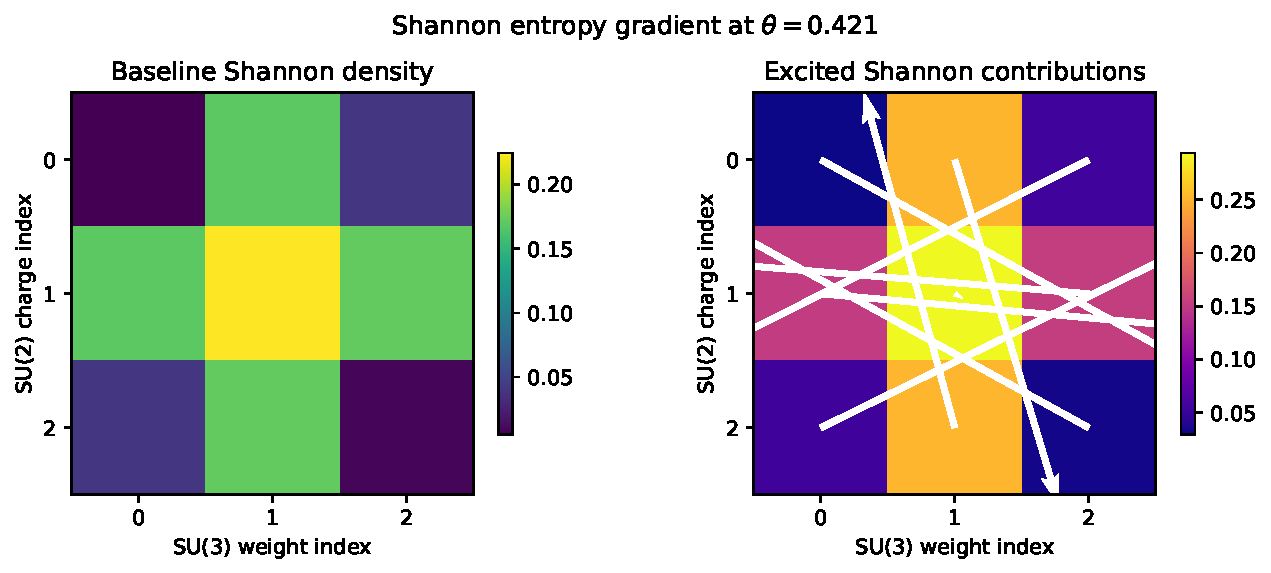
\includegraphics[width=0.86\columnwidth]{figures/entropy_gradient.pdf}
  \caption{Baseline and phase-locked Shannon contributions at
  \(\theta=\SimOutputPhaseTheta\).  The arrows display the discrete gradient
  of the excited entropy contribution.}\label{fig:entropy-gradient}
\end{figure}

\subsection{Directional entropy shear}

Order the nine coordinates by a fixed sequence
\begin{equation}
  \sigma
  =
  (c_1,c_2,\ldots,c_9),
  \qquad
  c_m\in\mathcal C,
  \label{eq:ordered-visible-sequence}
\end{equation}
and fold that sequence onto the prime skeleton
\begin{equation}
  (p_0,p_1,p_2,p_3,p_4)
  =
  (2,3,5,7,11),
  \qquad
  x_r^{(p)}
  =
  \ln p_r.
  \label{eq:prime-skeleton}
\end{equation}
Let \(\chi_m^{(x)}\) be the signed longitudinal character of coordinate \(c_m\), normalized so that \(|\chi_m^{(x)}|\leq1\).  At holographic resolution \(\tau\), the directional prime-load vector is
\begin{equation}
  \ell_r^{(x)}(\theta,\boldsymbol{x};\tau)
  =
  \frac{1}{1+\tau}
  \sum_{m=1}^{9}
  \rho_E^{(\theta)}(c_m)
  \left[
    1+
    \frac{x}{R_{\mathrm{bubble}}}
    \chi_m^{(x)}
  \right]
  \mathbb I_{\{m-1\equiv r\;(\mathrm{mod}\;5)\}},
  \qquad
  r=0,\ldots,4.
  \label{eq:directional-prime-load}
\end{equation}
The longitudinal Euler flux on the four prime intervals is then
\begin{equation}
  \Phi_s^{(x)}(\theta,\boldsymbol{x};\tau)
  =
  \frac{
    \ell_{s+1}^{(x)}(\theta,\boldsymbol{x};\tau)
    -
    \ell_s^{(x)}(\theta,\boldsymbol{x};\tau)
  }{
    \ln(p_{s+1}/p_s)
  },
  \qquad
  s=0,1,2,3.
  \label{eq:directional-entropy-shear}
\end{equation}
This quantity is the discrete boundary derivative that carries directional information into the bulk projector.  It vanishes for a load vector that is constant on the logarithmic prime lattice and changes sign under reversal of the longitudinal orientation.

Finally, the excitation remains on the fixed branch,
\begin{equation}
  \widehat{\mathcal O}_{\mathrm{excitation}}(\theta):
  \mathcal H_{\mathrm{vis}}(\mathfrak b_*)
  \longrightarrow
  \mathcal H_{\mathrm{vis}}(\mathfrak b_*),
  \qquad
  \delta k_\ell
  =
  \delta k_q
  =
  \delta K
  =
  0.
  \label{eq:branch-preserving-excitation}
\end{equation}
Since \(\Delta_{\mathrm{fr}}\) depends only on these discrete levels,
\begin{equation}
  \Delta_{\mathrm{fr}}(\theta)
  =
  \Delta_{\mathrm{fr}}(\mathfrak b_*)
  =
  0,
  \qquad
  \mathcal E_{\mu\nu}(\theta)
  =
  0
  \quad
  \text{for every admissible }\theta.
  \label{eq:framing-preserved-under-excitation}
\end{equation}